\section{Dokumentation \& Doxygen}
\subsection{Dokumentation}
\subsubsection{Zweck der Dokumentation}
\begin{itemize}
	\item Wissenssicherung / Wissenstransfer
	\item Kommunikation
	\item Sichtbarkeit des Projektfortschritts
\end{itemize}
\subsubsection{Dokumentation von Software}
\begin{minipage}{\linewidth}
\begin{itemize}
	\item Benutzung von bestehenden Programmteilen \newline $\rightarrow$ Schnittstellenbeschreibung (API, Application Program Interface)
	\item Zielgruppe ist Programmierer
	\item Dokumente werden oftmals nicht nachgeführt, wenn Änderungen am Sourcecode gemacht werden $\rightarrow$ Inkonsistenz \newline $\rightarrow$ Programmdokument ist fehlerhaft und verliert dadurch an Wert.
	\item Im Sourcecode wird mittels speziellem gekennzeichnetem Kommentar Beschreibung erstellt /** Text */
	\item Mittels Dokumentationswerkzeugen kann Kommentar Source-Code extrahiert werden und daraus eine Beschreibung erstellen.  
\end{itemize}
\end{minipage}
\subsection{Doxygen}
Doxygen ist ein solches Dokumentationswerkzeugen wie oben erwähnt. Es erstellt API-Beschreibungen.\\
Es ist weit verbreitet und Open-Source. (Beispiel im Anhang)
\begin{itemize}
	\item unterstütze Sprachen: C,C++,Java, C\#,...
	\item Ausgabeformate: HTML; LaTeX, RTF, XML,...
	\item auch UML-Diagramme möglich
	\item Ist grundsätzlich ein Command Line Tool
	\item Hauptbefehl (command-line): \texttt{\$ \textcolor{blue}{doxygen}}
	\item existiert aber auch ein GUI und ein Eclipse-Plugin (Eclox, in Eclipse das Symbol @)
	\item benötigt Konfigurationsdatei \"{}Doxyfile\"{} \newline
	 $\rightarrow$ \"{}Doxygen\"{} ist sehr umfangreich: rund 70.. 100 Optionen. \newline $\rightarrow$ Wichtigster Parameter: \texttt{PROJECT\_NAME} 
	\item im File Doxyfile sind alle Einstellungen gespeicher was alles in die Dokumentation muss
\end{itemize}
\begin{multicols}{2}
\subsubsection{Doxygen Commands}
\renewcommand{\arraystretch}{1.3}
\begin{minipage}{\linewidth}
\begin{tabular}{|l|l|}
	\hline	/** DoxyCmt */  &  Doxygen Comment\\ 
	\hline	@file	      	& File Name. Next Line Description of the File.\\
	\hline	@author 	    & Author\\
	\hline	@version	    & Version \\
	\hline   @date		    & Datum   \\ 
	\hline   @bug    		& A known Bug \\
	\hline   @brief	    	& One Line description  \\
	\hline   @extended	    & Description over several Lines  \\
	\hline   @param	       	& Description of your Parameter  \\
	\hline   @return	    & Description of your Returnvalue     \\ 
	\hline   @warning	    & Warnings \\ 
	\hline   @note		    & Note\\ 
	\hline        
\end{tabular}
\end{minipage}
\subsubsection{Aufruf-Beispiele}
\begin{minipage}{\linewidth}
\begin{itemize}
\item \texttt{doxygen} // gibt Hilfe-Text aus
\item \texttt{doxygen -g}           // erzeugt Konfig.-Datei \"{}Doxyfile\"{}
\item \texttt{doxygen Doxyfile}     // erzeugt Dokumentation
\end{itemize}
\end{minipage}
\end{multicols}
\clearpage
\subsubsection{Doxygen Architektur}
\vspace{3cm}
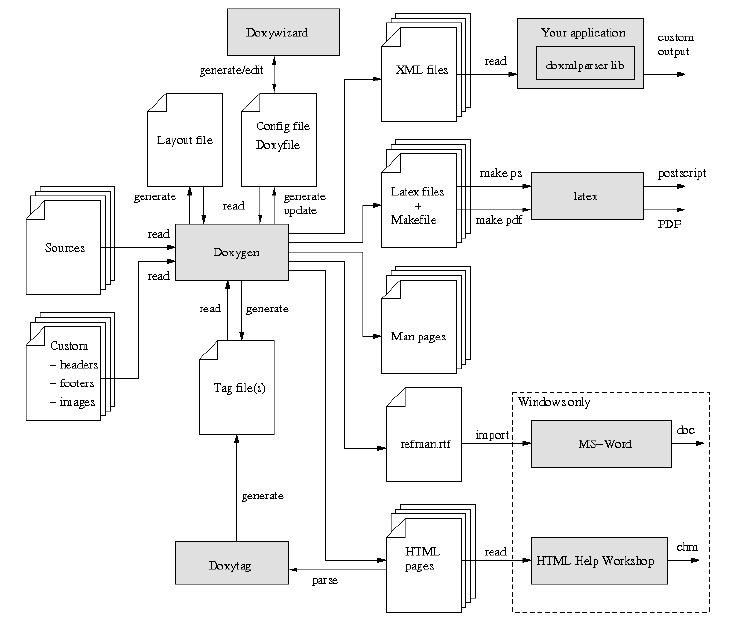
\includegraphics[width = \linewidth, angle = 90]{images/doxygen}
\clearpage
